\documentclass[tikz,border=8pt]{standalone}
\usepackage{amsmath,amssymb,xcolor}
\usetikzlibrary{arrows.meta,positioning}
\begin{document}
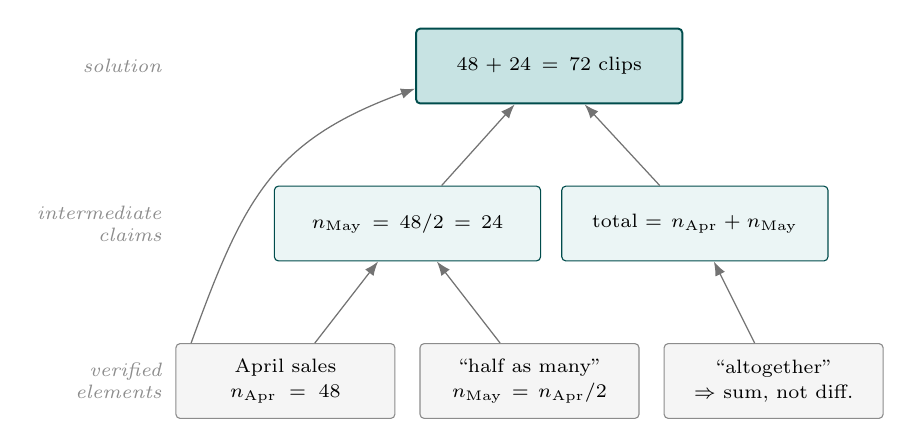
\begin{tikzpicture}[
  >={Latex[length=1.8mm]},
  edge/.style={->, line width=.45pt, draw=black!55},
  fact/.style={draw=black!45, fill=black!4, rounded corners=1.5pt,
               align=center, text width=2.5cm, inner sep=4pt,
               font=\scriptsize, minimum height=.95cm},
  claim/.style={draw=teal!60!black, fill=teal!8, rounded corners=1.5pt,
                align=center, text width=3.1cm, inner sep=4pt,
                font=\scriptsize, minimum height=.95cm},
  sol/.style={draw=teal!60!black, fill=teal!22, rounded corners=1.5pt,
              line width=.7pt, align=center, text width=3.1cm, inner sep=4pt,
              font=\scriptsize, minimum height=.95cm},
  tier/.style={font=\scriptsize\itshape, text=black!45, anchor=east, align=right}
]

% ---------- tier 0: verified elements ----------
\node[fact] (f1) at (0,0)   {April sales\\[1pt] $n_{\mathrm{Apr}} = 48$};
\node[fact] (f2) at (3.1,0) {``half as many''\\[1pt] $n_{\mathrm{May}} = n_{\mathrm{Apr}}/2$};
\node[fact] (f3) at (6.2,0) {``altogether''\\[1pt] $\Rightarrow$ sum, not diff.};

% ---------- tier 1: intermediate claims ----------
\node[claim] (c1) at (1.55,2.0) {$n_{\mathrm{May}} = 48/2 = 24$};
\node[claim] (c2) at (5.2,2.0)  {total $= n_{\mathrm{Apr}} + n_{\mathrm{May}}$};

% ---------- tier 2: solution ----------
\node[sol] (s) at (3.35,4.0) {$48 + 24 = 72$ clips};

% ---------- edges ----------
\draw[edge] (f1) -- (c1);
\draw[edge] (f2) -- (c1);
\draw[edge] (f3) -- (c2);
\draw[edge] (c1) -- (s);
\draw[edge] (c2) -- (s);
\draw[edge]
  ([xshift=2mm]f1.north west)
  to[out=70, in=-160, looseness=1.15]
  ([yshift=2mm]s.south west);

% ---------- tier labels ----------
\node[tier] at (-1.45,0)   {verified\\elements};
\node[tier] at (-1.45,2.0) {intermediate\\claims};
\node[tier, align=right] at (-1.45,4.0) {solution};


\end{tikzpicture}
\end{document}
